\documentclass[aspectratio=169,11pt]{beamer}

\usetheme{default}
\usecolortheme{default}
\usefonttheme{professionalfonts}
\usepackage[T1]{fontenc}
\renewcommand{\rmdefault}{lmr}\renewcommand{\sfdefault}{lmss}\renewcommand{\ttdefault}{lmtt}   % Latin Modern text, Computer Modern math
\usepackage{booktabs}
\usepackage{tikz}
\usetikzlibrary{arrows.meta,positioning,calc}

\definecolor{accent}{HTML}{2A78D6}
\definecolor{ink}{HTML}{0B0B0B}
\definecolor{muted}{HTML}{52514E}
\definecolor{boxblue}{HTML}{E8F1FC}
\definecolor{boxgreen}{HTML}{E7F6EF}
\definecolor{linegreen}{HTML}{1BAF7A}
\definecolor{boxorange}{HTML}{FDEEE7}
\definecolor{lineorange}{HTML}{EB6834}
\setbeamercolor{frametitle}{fg=accent}
\setbeamercolor{title}{fg=accent}
\setbeamercolor{normal text}{fg=ink}
\setbeamercolor{itemize item}{fg=accent}
\setbeamercolor{itemize subitem}{fg=muted}
\setbeamercolor{enumerate item}{fg=accent}
\setbeamertemplate{navigation symbols}{}
\setbeamertemplate{itemize items}[circle]
\setbeamerfont{frametitle}{series=\bfseries,size=\Large}
\setbeamertemplate{footline}{\hfill\textcolor{muted}{\scriptsize Krishna Jhanwar --- PrefEval final \quad \insertframenumber/\inserttotalframenumber}\hspace{0.4cm}\vspace{0.25cm}}

\newcommand{\nQuestions}{64,535}
\newcommand{\nCells}{65}
\newcommand{\nQuestionsRun}{64,478}
\newcommand{\gpuHours}{71}
\newcommand{\nCompared}{29}
\newcommand{\nWithinFive}{12}
\newcommand{\nWithinTen}{20}
\newcommand{\medianAbsDelta}{6.0}
\newcommand{\llamaSCemptyOneK}{25.2}
\newcommand{\llamaSCrtwZero}{205}
\newcommand{\llamaSCwtrZero}{51}
\newcommand{\llamaSCfirstZero}{94.4}
\newcommand{\mistralSCrtwZero}{188}
\newcommand{\mistralSCwtrZero}{29}
\newcommand{\mistralSCfirstZero}{95.6}
\newcommand{\posAccAthree}{60}
\newcommand{\posAccDthree}{43}
\newcommand{\posAccAlong}{42}
\newcommand{\posAccDlong}{23}
\newcommand{\posPickDthree}{14}
\newcommand{\posPickDlong}{8}
\newcommand{\llamaRagRefusalAll}{19.1}

\newcommand{\pRows}{12,950}
\newcommand{\pPos}{3,143}
\newcommand{\pNeg}{9,807}
\newcommand{\pGold}{3,580}
\newcommand{\pPseudo}{9,188}
\newcommand{\pAudited}{182}
\newcommand{\pDupDropped}{1,553}
\newcommand{\pPrefevalTurns}{8,757}
\newcommand{\pOasstPool}{15,427}
\newcommand{\pOasstRev}{fdf72ae0}
\newcommand{\pPersonaFound}{998}
\newcommand{\pOverlapAgree}{95.3}
\newcommand{\pOasstYes}{289}
\newcommand{\pStrictConfirmed}{115}
\newcommand{\pStrictRejected}{174}
\newcommand{\pGenericExcl}{1,384}
\newcommand{\pStrictExcl}{791}
\newcommand{\pGenericPrec}{0.28}
\newcommand{\pStrictPrec}{0.60}
\newcommand{\pAuditBefore}{73.9}
\newcommand{\pAuditAfter}{90.7}
\newcommand{\pKappa}{0.48}
\newcommand{\pTopicRateLo}{0.35}
\newcommand{\pTopicRateHi}{0.41}
\newcommand{\pFOneLo}{0.969}
\newcommand{\pFOneHi}{0.976}
\newcommand{\pBestEnsFOne}{0.977}
\newcommand{\pBestEnsMembers}{TinyLlama + Qwen3}
\newcommand{\pErrCorrLo}{0.68}
\newcommand{\pErrCorrHi}{0.75}
\newcommand{\pDisagreeMax}{0.9}
\newcommand{\pLlmFOne}{0.879}
\newcommand{\pLlmPrec}{0.787}
\newcommand{\pLlmRec}{0.996}
\newcommand{\pLlmFpr}{16.5}
\newcommand{\pLlmLat}{72}
\newcommand{\pDistilLat}{1.4}
\newcommand{\pSpeedup}{51}
\newcommand{\pDistilSameFOne}{0.990}
\newcommand{\pOodLo}{0.1}
\newcommand{\pOodHi}{1.5}
\newcommand{\pTotalTrainH}{4.3}
\newcommand{\pOasstRecLo}{16}
\newcommand{\pOasstRecHi}{26}
\newcommand{\pOasstPosTest}{114}

\newcommand{\qSimExR}{40.0}
\newcommand{\qGemExR}{82.7}
\newcommand{\qSimImR}{58.5}
\newcommand{\qGemImR}{87.7}
\newcommand{\qSimExROne}{8.5}
\newcommand{\qGemExROne}{82.4}
\newcommand{\qGemLat}{15.6}
\newcommand{\qMxbaiExR}{77.9}
\newcommand{\qEFiveExR}{30.7}
\newcommand{\qReplyGap}{0.6}
\newcommand{\qMemEx}{98.6}
\newcommand{\qMemIm}{99.9}
\newcommand{\qFalseSixteen}{0.22}
\newcommand{\qFalseTwentyThree}{0.65}
\newcommand{\qMissedEx}{14}
\newcommand{\qLlExMemThree}{96.5}
\newcommand{\qLlExRagThree}{74.8}
\newcommand{\qLlImMemThree}{83.5}
\newcommand{\qLlImRagThree}{73.7}
\newcommand{\qLlExGemThree}{93.9}
\newcommand{\qMiMemTwentyThree}{88.6}
\newcommand{\qMiRagTwentyThree}{53.7}
\newcommand{\qMiRemTwentyThree}{46.9}
\newcommand{\qMiZsTwentyThree}{37.6}
\newcommand{\qMiMemTen}{93.7}
\newcommand{\qMiGainTwentyThree}{34.9}
\newcommand{\qMiImMemZero}{81.9}
\newcommand{\qMiImRemZero}{88.4}
\newcommand{\qMiImMemThree}{79.8}
\newcommand{\qMiImRagThree}{64.0}
\newcommand{\qLostEx}{49}
\newcommand{\qLostExParse}{40}
\newcommand{\qLostIm}{99}
\newcommand{\qLostImParse}{65}
\newcommand{\qLostImGold}{98}
\newcommand{\qMiCondTen}{94.5}
\newcommand{\qMiCondTwentyThree}{89.1}
\newcommand{\qMiMissAccLo}{36}
\newcommand{\qMiMissAccHi}{50}
\newcommand{\qStExAll}{90.5}
\newcommand{\qStExTop}{93.9}
\newcommand{\qStImAll}{71.1}
\newcommand{\qStImTop}{77.0}
\newcommand{\qStKeepEx}{97.4}
\newcommand{\qStKeepIm}{98.5}
\newcommand{\qTokZs}{3,282}
\newcommand{\qTokMem}{3,343}
\newcommand{\qTokAdd}{61}
\newcommand{\qClfLat}{1.4}
\newcommand{\qTotalQ}{46,000}
\newcommand{\qGpuHours}{44}

\graphicspath{{figures/}{../results/phase2/figures/}}

\newcommand{\takeaway}[1]{\vspace{4pt}\begin{beamercolorbox}[sep=6pt,rounded=true]{normal text}\colorbox{boxblue}{\parbox{0.93\linewidth}{\small #1}}\end{beamercolorbox}}

\tikzset{
  box/.style={draw=accent, fill=boxblue, rounded corners=2pt, align=center, inner sep=3pt, minimum height=8mm},
  gbox/.style={draw=linegreen, fill=boxgreen, rounded corners=2pt, align=center, inner sep=3pt, minimum height=8mm},
  obox/.style={draw=lineorange, fill=boxorange, rounded corners=2pt, align=center, inner sep=3pt, minimum height=8mm},
  arr/.style={-{Stealth[length=1.8mm]}, thick, draw=black!70}}

\title{Improving Long-Context Preference Following in LLMs}
\subtitle{via a Trained Preference-Detection Classifier and Enhanced Retrieval}
\author{Krishna Jhanwar (12341250)}
\date{November 2026}

\begin{document}

\begin{frame}[plain]
\titlepage
\end{frame}

%-------------------------------------------------------------------------------
\begin{frame}{The problem: LLMs forget what you told them}
\begin{center}
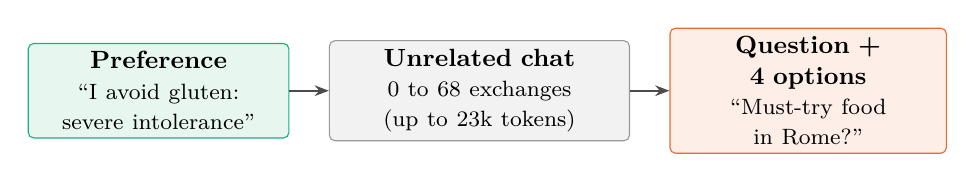
\begin{tikzpicture}[font=\small, node distance=3mm and 5mm]
\node[gbox, text width=3.1cm] (p) {\textbf{Preference}\\\footnotesize ``I avoid gluten: severe intolerance''};
\node[box, right=of p, text width=3.6cm, fill=black!5, draw=black!40] (c) {\textbf{Unrelated chat}\\\footnotesize 0 to 68 exchanges (up to 23k tokens)};
\node[obox, right=of c, text width=3.3cm] (q) {\textbf{Question + 4 options}\\\footnotesize ``Must-try food in Rome?''};
\draw[arr] (p) -- (c); \draw[arr] (c) -- (q);
\end{tikzpicture}
\end{center}
\vspace{2pt}
\begin{columns}[T]
\begin{column}{0.52\textwidth}
\textbf{PrefEval} (ICLR 2025)
\begin{itemize}\small
  \item 1{,}000 preference--question pairs, 20 topics
  \item Exactly one option respects the preference
  \item \emph{Explicit}: stated directly. \emph{Implicit}: revealed by choosing among options
\end{itemize}
\end{column}
\begin{column}{0.46\textwidth}
\textbf{Reproduced locally}
\begin{itemize}\small
  \item Llama zero-shot: 94.2\% at 0.2k $\rightarrow$ 43.3\% at 3k
  \item Mistral zero-shot: 95.5\% $\rightarrow$ \qMiZsTwentyThree\% at 23k
  \item Paper's best method (RAG), Mistral 23k: \qMiRagTwentyThree\%
\end{itemize}
\end{column}
\end{columns}
\takeaway{\textbf{Goal:} keep following preferences in long conversations, with open 7--8B models on one consumer GPU (RTX 3060, 12\,GB).}
\end{frame}

%-------------------------------------------------------------------------------
\begin{frame}{Proposed pipeline, and what is new}
\begin{center}
\resizebox{0.94\linewidth}{!}{%
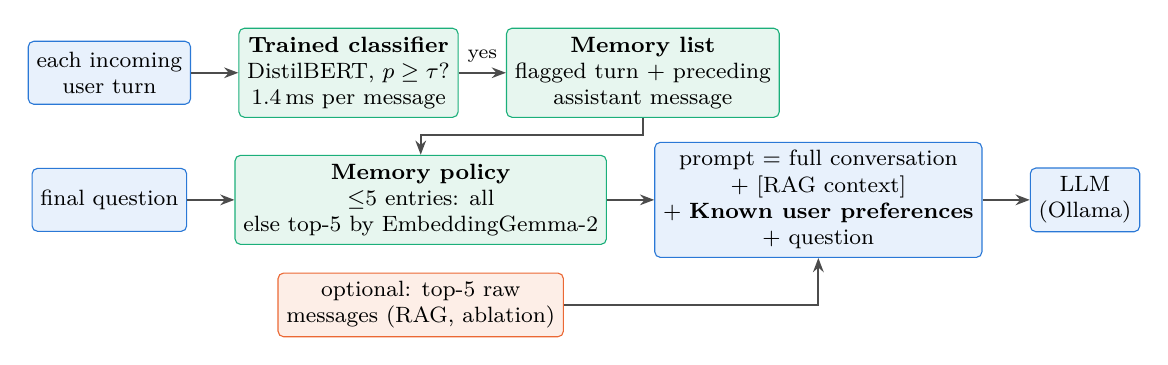
\begin{tikzpicture}[font=\footnotesize, node distance=3.5mm and 6mm]
\node[box] (turn) {each incoming\\user turn};
\node[gbox, right=of turn] (clf) {\textbf{Trained classifier}\\DistilBERT, $p \geq \tau$?\\\qClfLat\,ms per message};
\node[gbox, right=of clf] (mem) {\textbf{Memory list}\\flagged turn + preceding\\assistant message};
\node[box, below=8mm of turn] (q) {final question};
\node[gbox, right=of q] (sel) {\textbf{Memory policy}\\$\leq$5 entries: all\\else top-5 by EmbeddingGemma-2};
\node[obox, below=of sel] (rag) {optional: top-5 raw\\messages (RAG, ablation)};
\node[box, right=of sel] (prompt) {prompt = full conversation\\+ [RAG context]\\+ \textbf{Known user preferences}\\+ question};
\node[box, right=of prompt] (llm) {LLM\\(Ollama)};
\draw[arr] (turn) -- (clf);
\draw[arr] (clf) -- node[above, font=\scriptsize]{yes} (mem);
\draw[arr] (mem.south) |- ($(sel.north)+(0,2.5mm)$) -- (sel.north);
\draw[arr] (q) -- (sel);
\draw[arr] (sel) -- (prompt);
\draw[arr] (rag.east) -| (prompt.south);
\draw[arr] (prompt) -- (llm);
\end{tikzpicture}}
\end{center}
\textbf{What is new compared with the baselines}
\begin{itemize}\small
  \item All 5 baselines re-read the conversation at question time and keep \textbf{no state}; none has a trained component
  \item A \textbf{cheap trained gate} decides what to store: one forward pass, no extra LLM call
  \item Modern retriever benchmarked against the paper's 2021 SimCSE, and tested \emph{with and without} memory
\end{itemize}
\end{frame}

%-------------------------------------------------------------------------------
\begin{frame}{Phase 1: local reproduction of the baselines}
\begin{columns}[c]
\begin{column}{0.68\textwidth}
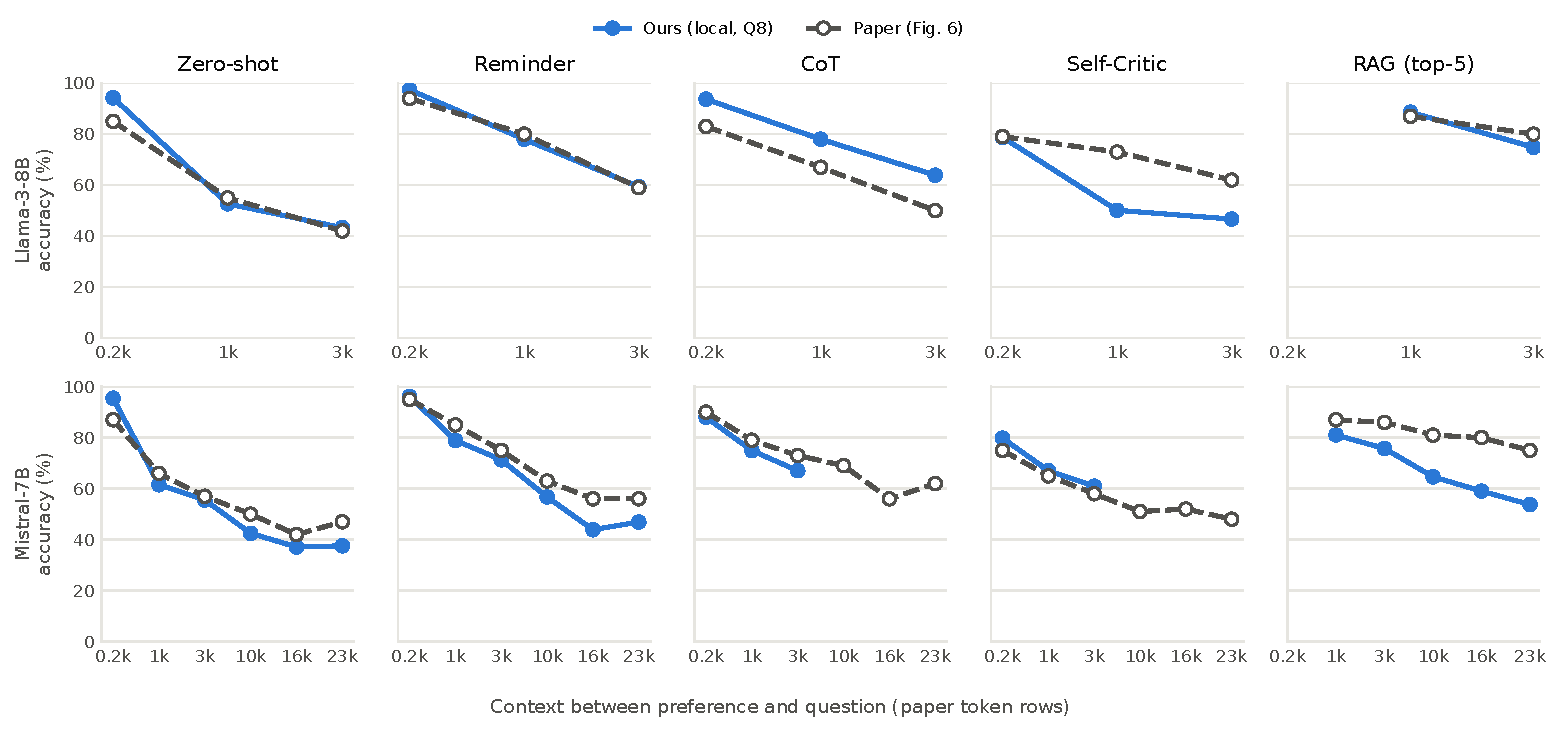
\includegraphics[width=\linewidth]{fig_vs_paper.pdf}
\end{column}
\begin{column}{0.31\textwidth}
\begin{itemize}\footnotesize
  \item Original prompts kept; only the inference call replaced (Bedrock $\rightarrow$ Ollama)
  \item \nQuestions{} questions, about \gpuHours{} GPU-hours
  \item \nWithinFive{} of \nCompared{} cells within 5 points of the paper, \nWithinTen{} within 10
  \item Fixed: double start token, whitespace bug, silent truncation, broken RAG files
\end{itemize}
\end{column}
\end{columns}
\takeaway{Trends reproduce. Largest gap: Mistral RAG at long context (53.7\% vs 75\%). The 8-bit KV cache is a plausible cause, not yet verified.}
\end{frame}

%-------------------------------------------------------------------------------
\begin{frame}{Phase 2: how the training data was built}
\begin{columns}[T]
\begin{column}{0.52\textwidth}
\centering\textbf{\pRows{} user messages}\\[3pt]
\resizebox{\linewidth}{!}{\begin{tabular}{llrrr}
\toprule
Source & Label origin & Label 1 & Label 0 & Rows \\
\midrule
Explicit preference & gold & 988 & 0 & 988 \\
Persona preference field & gold & 30 & 0 & 30 \\
Choice selection (implicit) & gold & 991 & 0 & 991 \\
Persona dialogue turn & pseudo (LLM) & 1,020 & 3,355 & 4,375 \\
Choice initial query & gold & 0 & 577 & 577 \\
Final question & gold & 0 & 994 & 994 \\
OpenAssistant message & pseudo (LLM) & 114 & 4,881 & 4,995 \\
\midrule Total & & 3,143 & 9,807 & 12,950 \\
\bottomrule
\end{tabular}
}
\end{column}
\begin{column}{0.46\textwidth}
\centering\textbf{Manual audit of pseudo-labels}\\[3pt]
\resizebox{\linewidth}{!}{\begin{tabular}{lrrr}
\toprule
Audit stratum & $n$ & Before refinement & After refinement \\
\midrule
Persona, LLM-picked turn (+) & 40 & 1.000 & 1.000 \\
Persona, other turns (-) & 39 & 0.821 & 0.966 \\
Persona, LLM vs overlap disagree & 40 & 0.475 & 0.909 \\
OpenAssistant, LLM yes (+) & 40 & 0.400 & 0.675 \\
OpenAssistant, LLM no (-) & 40 & 1.000 & 1.000 \\
\midrule All strata & 199 & 0.739 ($\kappa$=0.48) & 0.907 \\
\bottomrule
\end{tabular}
}
\end{column}
\end{columns}
\vspace{4pt}
\begin{itemize}\footnotesize
  \item \textbf{Gold} labels from PrefEval's structure; \textbf{pseudo}-labels from Llama-3-8B for persona turns and OpenAssistant
  \item Audit: OpenAssistant ``yes'' labels only 40\% correct (task requirements mistaken for preferences)
  \item Fixes: stricter re-check (174 rejected rows kept as hard negatives); union of LLM and word-overlap picks
\end{itemize}
\takeaway{The audit caught systematic label errors before training. Agreement: \pAuditBefore\% $\rightarrow$ \pAuditAfter\%.}
\end{frame}

%-------------------------------------------------------------------------------
\begin{frame}{Phase 2: how the classifiers were trained}
\begin{columns}[T]
\begin{column}{0.55\textwidth}
\textbf{Transfer learning}
\begin{itemize}\footnotesize
  \item Pretrained body + new 2-class head; input = message text only
  \item Cross-entropy loss, AdamW, warmup then linear decay
  \item Keep the checkpoint with best validation F1; early stopping
\end{itemize}
\vspace{2pt}
\resizebox{\linewidth}{!}{%
\begin{tabular}{lll}
\toprule
 & DistilBERT, ModernBERT & TinyLlama, Qwen3 \\
\midrule
Training & full fine-tuning & LoRA ($r{=}16$) + head \\
Trainable & 100\% & about 1\% \\
LR & 3e-5, 5e-5 & 2e-4 \\
Epochs, batch & 4, 32 & 2, 16$\times$2 \\
\bottomrule
\end{tabular}}
\end{column}
\begin{column}{0.43\textwidth}
\textbf{Leakage control: topic 5-fold CV}\\[4pt]
\centering
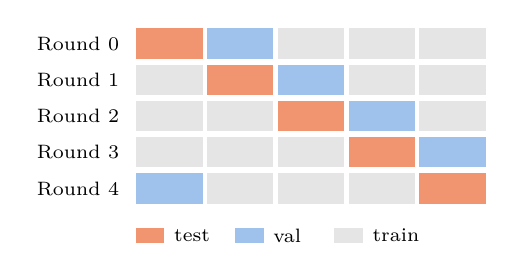
\begin{tikzpicture}[x=9mm,y=4.6mm,font=\scriptsize]
\foreach \r in {0,...,4}{
  \node[anchor=east] at (-0.1,-\r) {Round \r};
  \foreach \c in {0,...,4}{
    \pgfmathtruncatemacro{\v}{mod(\r+1,5)}
    \ifnum\c=\r \fill[lineorange!70] (\c,-\r-0.42) rectangle (\c+0.94,-\r+0.42);
    \else\ifnum\c=\v \fill[accent!45] (\c,-\r-0.42) rectangle (\c+0.94,-\r+0.42);
    \else \fill[black!10] (\c,-\r-0.42) rectangle (\c+0.94,-\r+0.42); \fi\fi
  }
}
\fill[lineorange!70] (0,-5.5) rectangle (0.4,-5.1); \node[anchor=west] at (0.4,-5.3) {test};
\fill[accent!45] (1.4,-5.5) rectangle (1.8,-5.1); \node[anchor=west] at (1.8,-5.3) {val};
\fill[black!10] (2.8,-5.5) rectangle (3.2,-5.1); \node[anchor=west] at (3.2,-5.3) {train};
\end{tikzpicture}
\vspace{2pt}
\begin{itemize}\footnotesize
  \item 4 topics per fold; test topics unseen in training
  \item LMSYS distractors never trained on
\end{itemize}
\end{column}
\end{columns}
\takeaway{4 models $\times$ 5 folds = 20 trainings, \pTotalTrainH{} hours in total. Both leakage rules are asserted in code.}
\end{frame}

%-------------------------------------------------------------------------------
\begin{frame}{Phase 2: classifier results}
\centering
\resizebox{\linewidth}{!}{\begin{tabular}{lrrrrrrrrrr}
\toprule
Model & F1 & Prec. & Rec. & F1 std & AUC & ECE & OOD flags & ms/msg & Trainable & Train min \\
\midrule
DistilBERT & 0.969 & 0.983 & 0.955 & 0.007 & 0.994 & 0.008 & 0.4\% & 1.4 & 67M & 14 \\
ModernBERT & 0.972 & 0.988 & 0.956 & 0.004 & 0.995 & 0.009 & 0.2\% & 6.5 & 150M & 32 \\
TinyLlama-1.1B (LoRA) & 0.974 & 0.988 & 0.961 & 0.006 & 0.997 & 0.010 & 0.1\% & 17.1 & 13M & 91 \\
Qwen3-1.7B (LoRA) & 0.976 & 0.988 & 0.965 & 0.006 & 0.997 & 0.009 & 1.5\% & 25.1 & 17M & 120 \\
\bottomrule
\end{tabular}
}
\vspace{6pt}
\begin{columns}[T]
\begin{column}{0.48\textwidth}
\textbf{vs prompted LLM} (same 2{,}000 rows)\\[3pt]
\resizebox{\linewidth}{!}{%
\begin{tabular}{lcccc}
\toprule
Detector & F1 & Prec. & Rec. & ms/msg \\
\midrule
Prompted Llama-3-8B & \pLlmFOne & \pLlmPrec & \pLlmRec & \pLlmLat \\
\textbf{DistilBERT} & \textbf{\pDistilSameFOne} & 0.991 & 0.990 & \textbf{\pDistilLat} \\
\bottomrule
\end{tabular}}
\end{column}
\begin{column}{0.5\textwidth}
\begin{itemize}\footnotesize
  \item All four within 0.7 F1 points; Qwen3 is best, but 18$\times$ slower
  \item Best of 33 ensembles: \pBestEnsFOne, only +0.001, because errors are correlated (0.68--0.75)
  \item Limitation: casual real-chat recall only \pOasstRecLo--\pOasstRecHi\%
\end{itemize}
\end{column}
\end{columns}
\takeaway{\textbf{DistilBERT selected:} \pSpeedup$\times$ faster than the LLM, more accurate, and low false alarms on the distractor turns.}
\end{frame}

%-------------------------------------------------------------------------------
\begin{frame}{Phase 3, Step 1: which encoder finds the preference?}
\begin{columns}[c]
\begin{column}{0.6\textwidth}
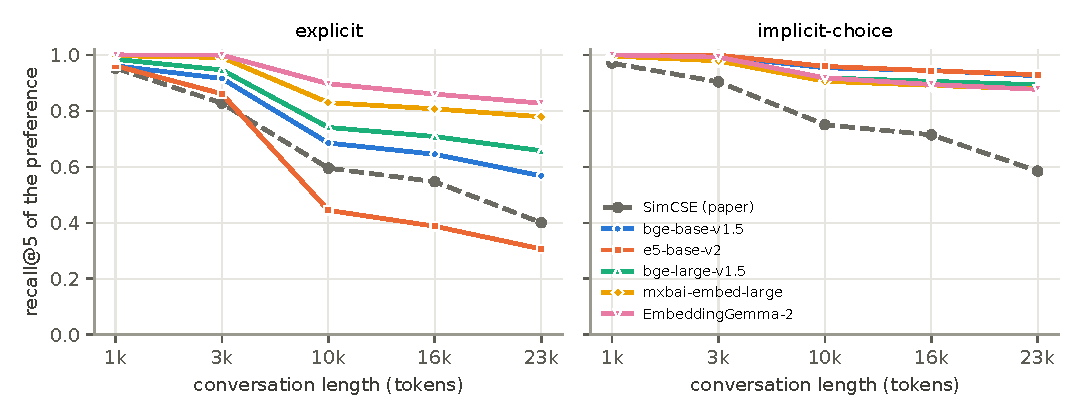
\includegraphics[width=\linewidth]{p3_retrieval.pdf}
\end{column}
\begin{column}{0.39\textwidth}
\begin{itemize}\scriptsize
  \item SimCSE at 23k: \qSimExR\% $\rightarrow$ EmbeddingGemma-2: \qGemExR\% (explicit)
  \item SimCSE ranks the preference first only \qSimExROne\% of the time at 1k
  \item e5-base is \emph{worse} than SimCSE on long explicit (\qEFiveExR\%)
  \item Nobody ranks an implicit selection first $\rightarrow$ store it \emph{with} its options
\end{itemize}
\end{column}
\end{columns}
\vspace{2pt}
\centering
\resizebox{0.8\linewidth}{!}{\begin{tabular}{lr|ccccc|cccc|r}
\toprule
 & & \multicolumn{5}{c|}{Explicit} & \multicolumn{4}{c|}{Implicit-choice} &  \\
Retriever & Params & R@5 1k & 3k & 10k & 23k & R@1 23k & R@5 1k & 3k & 10k & 23k & ms/msg \\
\midrule
SimCSE (paper) & 355M & 0.95 & 0.83 & 0.60 & 0.40 & 0.05 & 0.97 & 0.90 & 0.75 & 0.58 & -- \\
\midrule
bge-base-v1.5 & 110M & 0.96 & 0.92 & 0.68 & 0.57 & 0.29 & 1.00 & 0.99 & 0.95 & 0.92 & 3.5 \\
e5-base-v2 & 110M & 0.96 & 0.86 & 0.44 & 0.31 & 0.12 & 1.00 & 1.00 & 0.96 & 0.93 & 3.6 \\
bge-large-v1.5 & 335M & 0.98 & 0.95 & 0.74 & 0.66 & 0.43 & 1.00 & 0.99 & 0.92 & 0.89 & 9.8 \\
mxbai-embed-large & 335M & 1.00 & 0.99 & 0.83 & 0.78 & 0.53 & 1.00 & 0.98 & 0.91 & 0.88 & 9.8 \\
\textbf{EmbeddingGemma-2} & 744M & 1.00 & 1.00 & 0.90 & 0.83 & 0.53 & 1.00 & 0.99 & 0.92 & 0.88 & 15.6 \\
\bottomrule
\end{tabular}
}
\end{frame}

%-------------------------------------------------------------------------------
\begin{frame}[fragile]{Phase 3, Step 2: the preference memory}
\begin{columns}[T]
\begin{column}{0.45\textwidth}
\textbf{How it works}
\begin{itemize}\footnotesize
  \item Score each user message with a model that never saw its topic
  \item Store flagged turn + preceding assistant message
\end{itemize}
\textbf{Quality}
\begin{itemize}\footnotesize
  \item Preference caught: \textbf{\qMemEx\%} explicit, \textbf{\qMemIm\%} implicit
  \item False entries: none up to 10k, \qFalseTwentyThree{} per question at 23k
  \item Adds about \qTokAdd{} prompt tokens (Llama, explicit, 3k)
\end{itemize}
\end{column}
\begin{column}{0.53\textwidth}
\textbf{What the LLM sees} (implicit, shortened)\\[3pt]
\colorbox{boxgreen}{\parbox{0.96\linewidth}{\scriptsize\ttfamily
Known user preferences: these are the preferences I have stated before.\\[2pt]
\#Start of Known Preferences\#\\
{}[Preference 1, turn 2]\\
Assistant: There are many great hotel options in Las Vegas\ldots\\
User: I think I'll go with The Westin. The others seem too lively.\\
\#End of Known Preferences\#\\[2pt]
Please follow these preferences wherever they are relevant to my question.\\[2pt]
<question + 4 options>}}
\end{column}
\end{columns}
\takeaway{\textbf{Design rule:} each new method changes one thing from a baseline (96 prompts verified byte-for-byte against Phase~1).}
\end{frame}

%-------------------------------------------------------------------------------
\begin{frame}{Main result: memory stays nearly flat as context grows}
\centering
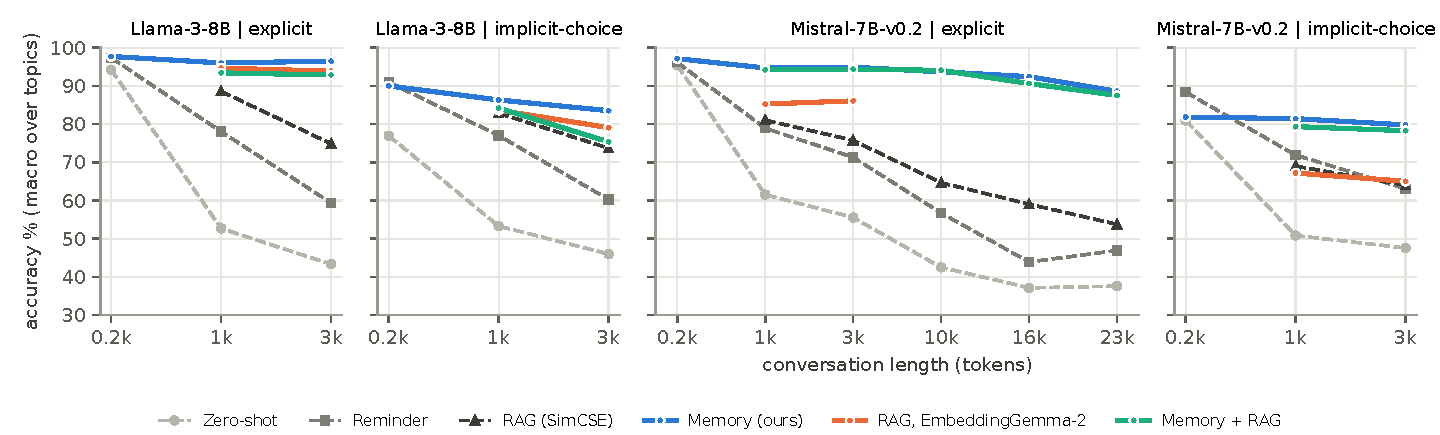
\includegraphics[width=\linewidth]{p3_main.pdf}
\takeaway{\textbf{Mistral at 23k: \qMiMemTwentyThree\% vs \qMiRagTwentyThree\%} for the paper's RAG, \qMiRemTwentyThree\% for Reminder, \qMiZsTwentyThree\% for zero-shot. From 0.2k to 23k, zero-shot and Reminder lose 49--58 points; memory loses 8.5.}
\end{frame}

%-------------------------------------------------------------------------------
\begin{frame}{Main result: the numbers}
\centering
\resizebox{0.88\linewidth}{!}{\begin{tabular}{lll|c|cc|c}
\toprule
Model & Form & Length & Best baseline & Memory & Memory + RAG & Gain \\
\midrule
Llama-3-8B & explicit & 3k & 74.8 (RAG) & \textbf{96.5} & 92.9 & +21.6 \\
Llama-3-8B & implicit-choice & 3k & 73.7 (RAG) & \textbf{83.5} & 75.4 & +9.8 \\
Mistral-7B-v0.2 & explicit & 3k & 75.7 (RAG) & \textbf{94.9} & 94.4 & +19.2 \\
Mistral-7B-v0.2 & explicit & 10k & 64.6 (RAG) & 93.7 & \textbf{94.1} & +29.1 \\
Mistral-7B-v0.2 & explicit & 16k & 59.0 (RAG) & \textbf{92.4} & 90.6 & +33.4 \\
Mistral-7B-v0.2 & explicit & 23k & 53.7 (RAG) & \textbf{88.6} & 87.5 & +34.9 \\
Mistral-7B-v0.2 & implicit-choice & 3k & 64.0 (RAG) & \textbf{79.8} & 78.3 & +15.8 \\
\bottomrule
\end{tabular}
}
\vspace{2pt}
\begin{itemize}\footnotesize
  \item Same questions, option order and strict metric as baselines; \qTotalQ{} questions, about \qGpuHours{} GPU-hours
  \item Beats every baseline in all 11 cells from 1k up; best overall in 10 (Mistral 10k: Memory + RAG is 0.4 higher)
  \item Also above the paper's published RAG: 80\% for Llama at 3k, 75\% for Mistral at 23k
\end{itemize}
\takeaway{\textbf{Exception:} at 0.2k there is nothing to forget. Memory ties Reminder on explicit, and loses on Mistral implicit (\qMiImMemZero\% vs \qMiImRemZero\%).}
\end{frame}

%-------------------------------------------------------------------------------
\begin{frame}{Ablation 1: swapping only the retriever}
\centering\small
\resizebox{0.9\linewidth}{!}{\begin{tabular}{lll|cc|c|c}
\toprule
Model & Form & Length & SimCSE RAG & EmbeddingGemma-2 RAG & $\Delta$ & Memory + RAG \\
\midrule
Llama-3-8B & explicit & 1k & 88.6 & 94.6 & +6.0 & 93.2 \\
Llama-3-8B & explicit & 3k & 74.8 & 93.9 & +19.1 & 92.7 \\
Llama-3-8B & implicit-choice & 1k & 82.8 & 84.1 & +1.2 & 84.5 \\
Llama-3-8B & implicit-choice & 3k & 73.7 & 79.6 & +6.0 & 75.8 \\
Mistral-7B-v0.2 & explicit & 1k & 81.0 & 85.5 & +4.5 & 94.2 \\
Mistral-7B-v0.2 & explicit & 3k & 75.7 & 86.3 & +10.6 & 94.5 \\
Mistral-7B-v0.2 & implicit-choice & 1k & 69.0 & 67.6 & -1.4 & 79.3 \\
Mistral-7B-v0.2 & implicit-choice & 3k & 64.0 & 65.6 & +1.6 & 78.2 \\
\bottomrule
\end{tabular}
}
\vspace{6pt}
\begin{itemize}\small
  \item Same prompt, same questions: only the encoder changes
  \item \textbf{Explicit improves strongly:} Llama at 3k goes from \qLlExRagThree{} to \qLlExGemThree
  \item \textbf{Implicit barely changes,} although retrieval itself improved: fragments of a dialogue are hard to use
\end{itemize}
\takeaway{A better encoder fixes the retrieval bottleneck for explicit preferences. Implicit needs the full options + selection context that memory provides.}
\end{frame}

%-------------------------------------------------------------------------------
\begin{frame}{Ablation 2: adding RAG on top of memory does not help}
\centering\small
\resizebox{\linewidth}{!}{\begin{tabular}{lll|cccc|c|c}
\toprule
Model & Form & Length & Lost & of which format & wrong option & pref.\ retrieved & Gained & Same answer \% \\
\midrule
Llama-3-8B & explicit & 3k & 49 & 40 & 9 & 49 & 11 & 93.8 \\
Llama-3-8B & implicit-choice & 3k & 99 & 65 & 34 & 98 & 16 & 85.2 \\
Mistral-7B-v0.2 & explicit & 3k & 14 & 0 & 14 & 14 & 7 & 97.5 \\
Mistral-7B-v0.2 & explicit & 23k & 28 & 0 & 28 & 22 & 16 & 95.1 \\
Mistral-7B-v0.2 & implicit-choice & 3k & 46 & 1 & 45 & 46 & 26 & 90.0 \\
\bottomrule
\end{tabular}
}
\vspace{6pt}
\begin{itemize}\small
  \item \textbf{Llama:} mostly format failures. It writes ``Based on your previous\ldots'' and the 5-token limit cuts it off (\qLostImParse{} of \qLostIm{} implicit losses)
  \item \textbf{Retrieval did not fail:} the preference was retrieved in \qLostImGold{} of those \qLostIm{}
  \item \textbf{Mistral:} its prompt pre-fills \texttt{<choice>}, so no format failures; same answer on 90--98\% of questions
\end{itemize}
\takeaway{With about 99\% classifier recall, there is little left for raw-message retrieval to recover. It mainly adds noise.}
\end{frame}

%-------------------------------------------------------------------------------
\begin{frame}{Ablation 3: what if memory holds many preferences?}
\begin{columns}[c]
\begin{column}{0.62\textwidth}
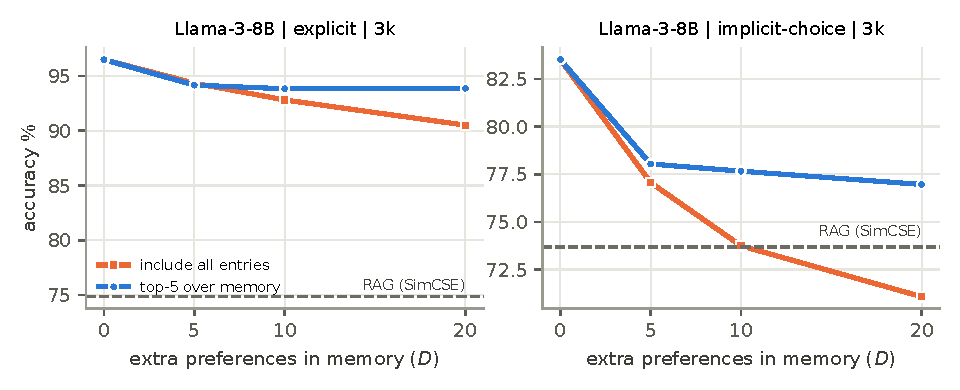
\includegraphics[width=\linewidth]{p3_stress.pdf}
\end{column}
\begin{column}{0.37\textwidth}
\centering\footnotesize
\resizebox{\linewidth}{!}{\begin{tabular}{lc|cc|cc}
\toprule
 & & \multicolumn{2}{c|}{Include all} & \multicolumn{2}{c}{Top-5 retrieval over memory} \\
Form & $D$ & entries & accuracy & pref.\ kept (\%) & accuracy \\
\midrule
explicit & 0 & 1 & 96.5 & 100.0 & 96.5 \\
 & 5 & 6 & \textbf{94.3} & 100.0 & 94.2 \\
 & 10 & 11 & 92.8 & 99.1 & \textbf{93.8} \\
 & 20 & 21 & 90.5 & 97.4 & \textbf{93.9} \\
\midrule
implicit-choice & 0 & 1 & 83.5 & 100.0 & 83.5 \\
 & 5 & 6 & 77.1 & 100.0 & \textbf{78.0} \\
 & 10 & 11 & 73.7 & 99.9 & \textbf{77.7} \\
 & 20 & 21 & 71.1 & 98.5 & \textbf{77.0} \\
\bottomrule
\end{tabular}
}
\end{column}
\end{columns}
\vspace{4pt}
\begin{itemize}\small
  \item Added $D$ preferences from \emph{other} topics, in random order (Llama, 3k tokens)
  \item Top-5 retrieval keeps the true preference for \qStKeepEx\% / \qStKeepIm\% of questions at $D{=}20$
\end{itemize}
\takeaway{\textbf{Retrieval is most useful over the memory:} at $D{=}20$, include-all falls to \qStExAll\% / \qStImAll\%; top-5 holds \qStExTop\% / \qStImTop\%.}
\end{frame}

\end{document}
